% a gem of a website: https://mpetroff.net/files/beamer-theme-matrix/
\documentclass[xcolor={dvipsnames,svgnames}]{beamer}
\usetheme{PaloAlto}
\usecolortheme{spruce}
\usepackage[utf8]{inputenc}
\usepackage{enumerate}
\usepackage{amsmath}
\usepackage{amsthm}
\usepackage{amssymb}
\usepackage{amsbsy}
\usepackage{amsfonts}
\usepackage{hyperref}
\usepackage{tikz}
\usepackage{verbatim}
\usepackage{mathtools}
\usepackage{macros}
\usepackage{float}
\usepackage{caption}
\usepackage{subcaption}
\usepackage{xcolor,graphicx}
\usepackage{animate}
\usepackage{tikz}
\usetikzlibrary{positioning}
\setbeamertemplate{caption}[numbered]
\DeclareUnicodeCharacter{2212}{-}
\usepackage{tikz-cd}
\usepackage{flowchart}
\usetikzlibrary{
  shapes,
  arrows.meta, % supersedes arrows
  calc,automata,positioning,fit,quotes}
  \tikzset{
  line/.style={draw, -Latex}
}
\tikzstyle{arrow} = [thick,->,>=stealth]
\captionsetup{font=scriptsize,labelfont={bf,sf}}
\captionsetup[subfigure]{font=scriptsize,labelfont=scriptsize}
\addtobeamertemplate{navigation symbols}{}{%
    \usebeamerfont{footline}%
    \usebeamercolor[fg]{footline}%
    \hspace{1em}%
    \insertframenumber/\inserttotalframenumber
}
\makeatletter
  \setbeamertemplate{sidebar \beamer@sidebarside}%{sidebar theme}
  {
    \beamer@tempdim=\beamer@sidebarwidth%
    \advance\beamer@tempdim by -6pt%
    \insertverticalnavigation{\beamer@sidebarwidth}%
    \vfill
    \ifx\beamer@sidebarside\beamer@lefttext%
    \else%
      \usebeamercolor{normal text}%
      \llap{\usebeamertemplate***{navigation symbols}\hskip0.1cm}%
      \vskip2pt%
    \fi%
}%
\title{Manifold Structure of High-Dimensional Data in Artificial and Biological Neural Networks}
\author{Zhang Liu\\ Supervisor: Francesca Spagnuolo \\ Co-supervisors: Steven W.~Zucker, Luciano Dyballa}

\date{\today}
% \logo{
\includegraphics[width=.075\textwidth]{YaleNUS_workmark_solid.eps}}
\begin{document}

\begin{frame}
\titlepage
\end{frame}

\section{Motivation}
\begin{frame}{Motivation: biological vision vs computer vision}
What is in common? What is different?

 \begin{minipage}[t]{.42\linewidth}  
    \begin{figure}
            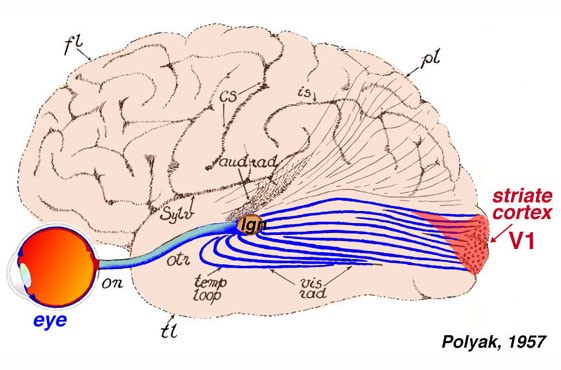
\includegraphics[width=0.75\textwidth]{presentation/figures-models/v1.jpg}
            \caption{Human brain.}
        \end{figure} 
    \end{minipage}
      \begin{minipage}[t]{.55\linewidth}   
      \begin{figure}         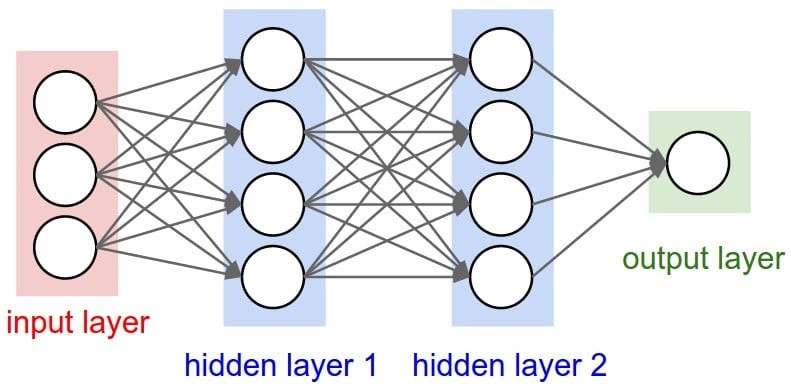
\includegraphics[width=0.8\textwidth]{presentation/figures-models/simple-ann.jpeg}
            \caption{Artificial Neural Network (ANN).}
            \end{figure} 
    \end{minipage}
    Brain and ANNs are instances of a black box problem! 
        \begin{figure}
            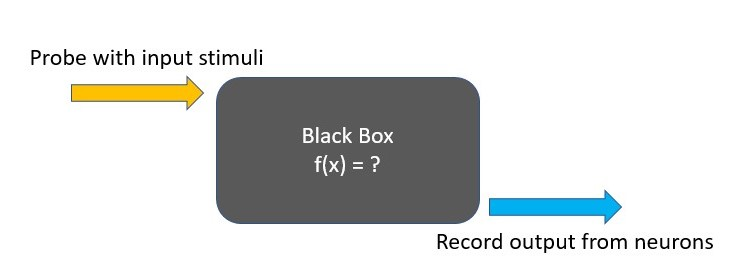
\includegraphics[width=0.85\textwidth]{presentation/figures-models/black-box.jpg}
        \end{figure} 
\end{frame}

\section{Method}
\begin{frame}{Previously:}
\begin{figure}[H]
        \centering
            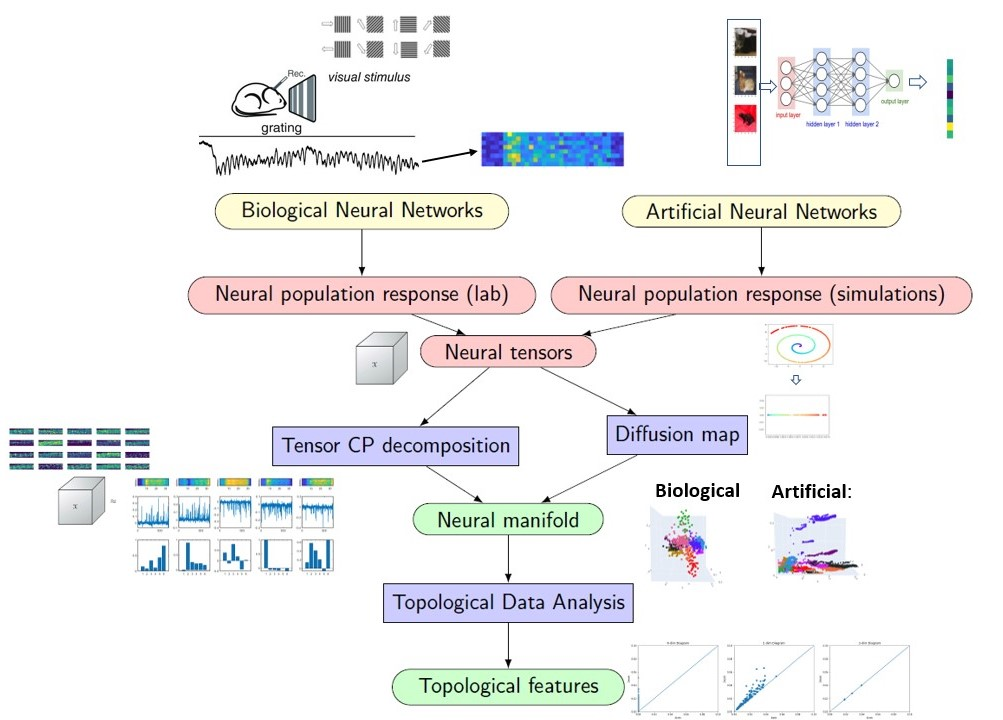
\includegraphics[width=\textwidth]{Slide4.jpg}
        \end{figure} 
\end{frame}

\begin{frame}{Framework for comparison}
  \begin{enumerate} 
  \item Probe with appropriate input stimuli.
  \item Obtain neuron output. This is our \textit{neural tensor}.
  \item With the algorithm we developed for each candidate network, we generate a \textit{neural manifold}. 
  
  (clusters of neurons grouped by their output patterns in response to a given input visual stimulus)
    \begin{itemize}
        \item Qualitative visualization: dimensionality reduction.
        \item Quantitative measure: mean flow ratio.
    \end{itemize}
 \end{enumerate}
 (In this presentation I will only give a high-level explanation for the algorithm. See actual capstone for details.)
\end{frame}

\begin{frame}{Framework for comparison}
    \begin{table}[]
\begin{tabular}{|l|l|l|}
\hline
              & Neurobiological & Computational     \\ \hline
Candidate    & Retina, V1      & CNN, RNN \\ 
Networks      &                 & Vision Transformer (ViT) \\\hline
Input stimuli & Flow stimuli \cite{visual-flow}  & ImageNet images \cite{deng2009imagenet} \\ \hline
Neuron output & Single-neuron   & Computational output \\ 
              & recording       & of neuron units \\ \hline
\end{tabular}
\end{table}

\begin{minipage}[t]{.45\linewidth}  
    \begin{figure}
            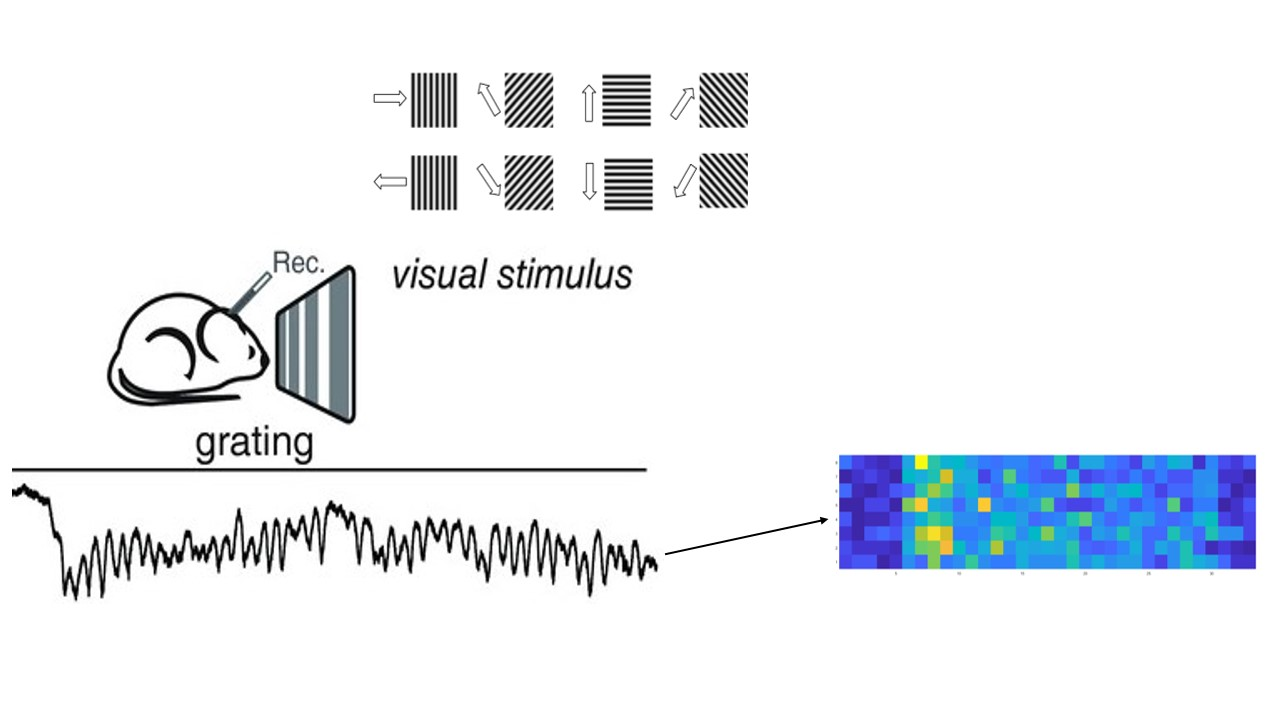
\includegraphics[width=\textwidth]{presentation/Slide5.jpg}
        \end{figure} 
    \end{minipage}
      \begin{minipage}[t]{.45\linewidth}   
      \begin{figure}         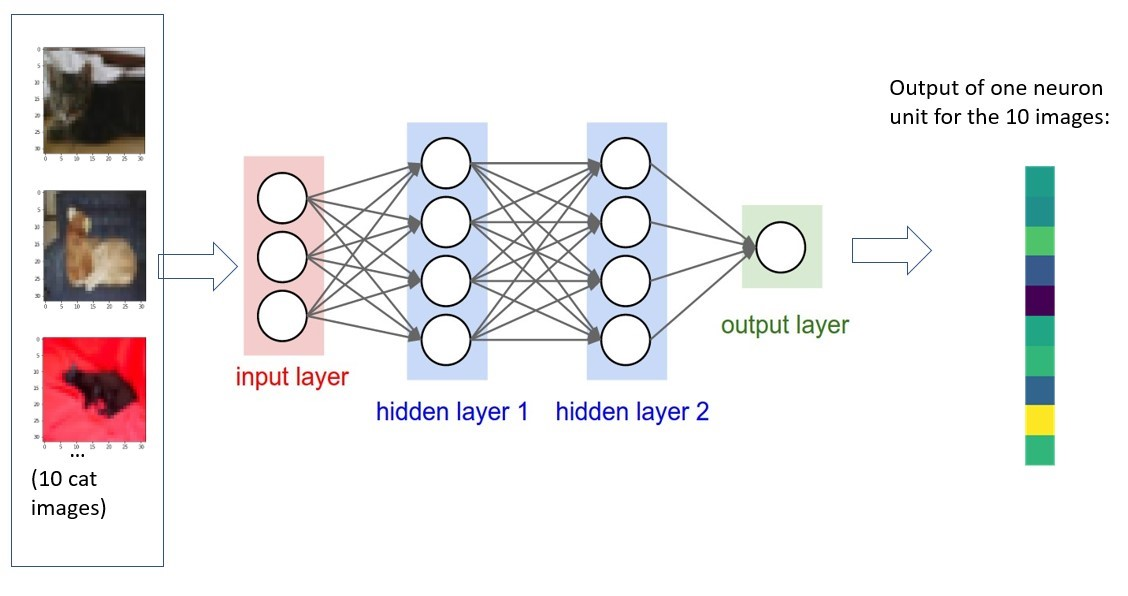
\includegraphics[width=\textwidth]{presentation/Slide1.jpg}
            \end{figure} 
    \end{minipage}
    
\end{frame}

\begin{frame}{Starting point: retina vs V1}
Neural manifold for V1 is much more continuous than that for the retina. 

\textbf{Questions:} How about the neural manifolds for computer vision models (ANNs)? Do they form continuous manifold like V1 or discontinuous clusters like the retina? 

    \begin{minipage}[t]{.45\linewidth}  
    \begin{figure}
            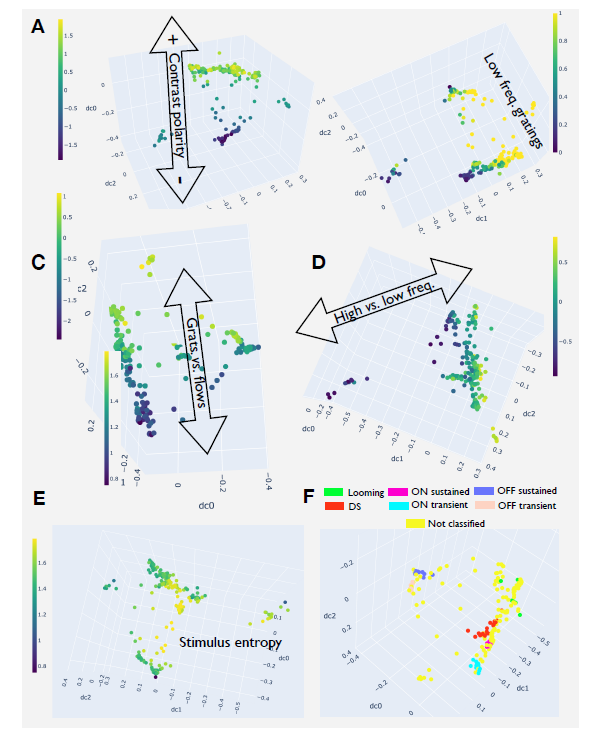
\includegraphics[width=0.6\textwidth]{presentation/embeddings/retina-manifold.PNG}
            \caption{Adapted from \cite{dyballa_manifold_2021}.}
        \end{figure} 
    \end{minipage}
      \begin{minipage}[t]{.45\linewidth}   
      \begin{figure}         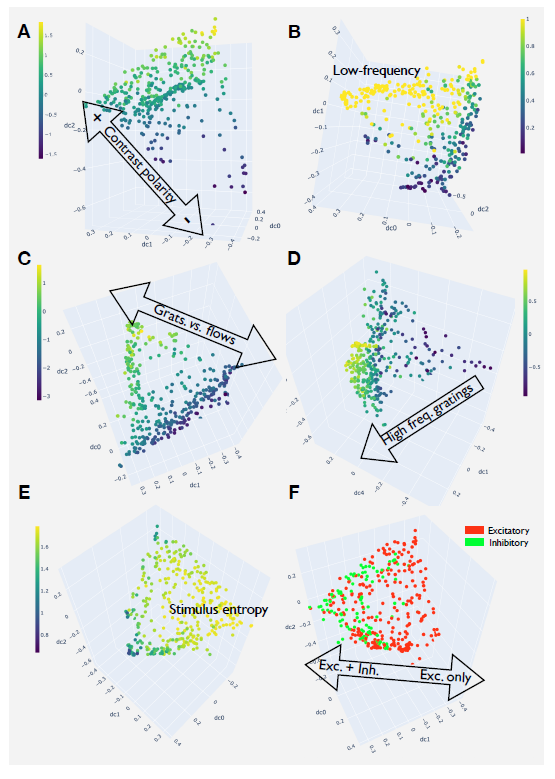
\includegraphics[width=0.55\textwidth]{presentation/embeddings/v1-manifold.PNG}
      \caption{Adapted from \cite{dyballa_manifold_2021}.}
            \end{figure} 
    \end{minipage}
\end{frame}

\begin{frame}{Dimensionality reduction: tensor CP decomposition}
Why? The neuron output is very high-dimensional and we cannot visualize their structure directly. 

We have to reduce the dimension to 3D to see how the neurons form clusters.
    \begin{figure}[H]
        \centering
            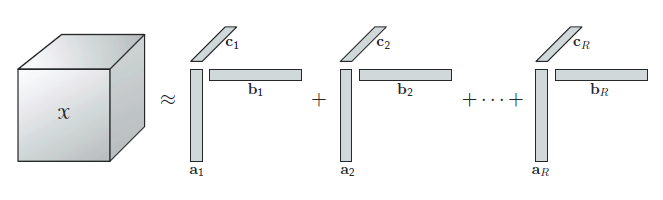
\includegraphics[width=0.8\textwidth]{figures-tensor/cp-decomp.png}
            \caption{Intuition for tensor CANDECOMP/PARAFAC (CP) decomposition. (Adapted from \cite{Kol2009}.)}
        \end{figure} 
\end{frame}
\begin{frame}{Mean flow ratio ($\phi_G$)}
Why? The mean flow ratio provides a quantifiable measure for how continuous the clusters of neurons are. This measure has its origin from the maximum flow problem. 
  \begin{figure}[H]
        \centering
         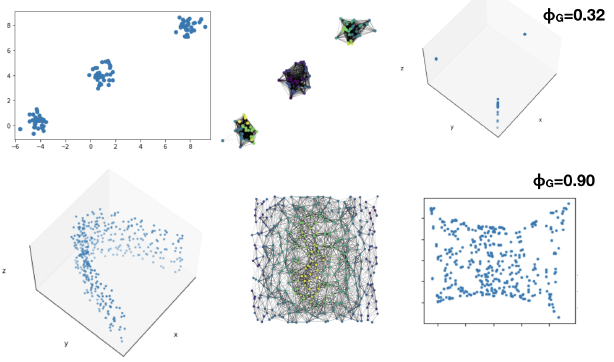
\includegraphics[width=0.8\textwidth]{presentation/embeddings/mean-flow-ratio.PNG}
            \caption{Intuition for mean flow ratio. (Adapted from \cite{dyballa_manifold_2021}.)}
        \end{figure} 
\end{frame}

\section{Results}

% \begin{frame}{Results: first five principal components from biological neural tensor}
%     \begin{figure}[H]
%         \centering
%             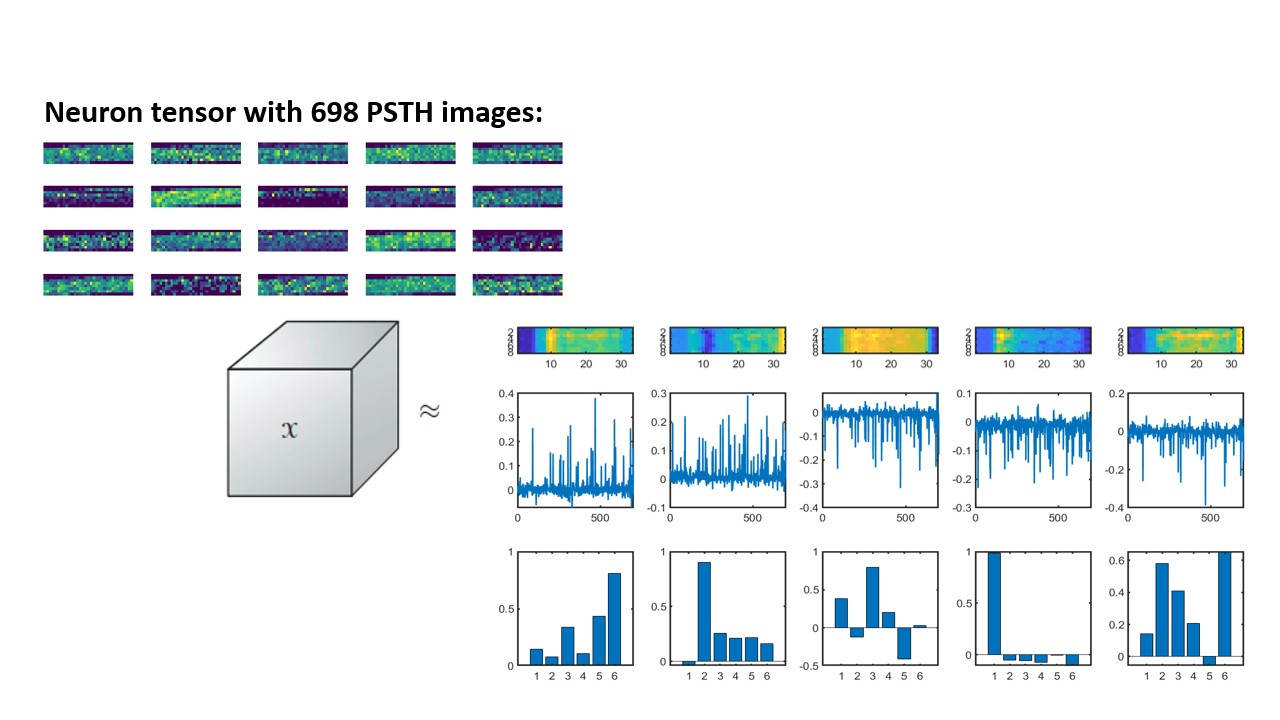
\includegraphics[width=\textwidth]{Slide3.jpg}
%             \caption{First 5 tensor factors for neural data.}
%         \end{figure} 
% \end{frame}

\begin{frame}{CNN: VGG16 structure}
The key operation in CNN is \textit{convolution}. 
     \begin{figure}[H]
        \centering
            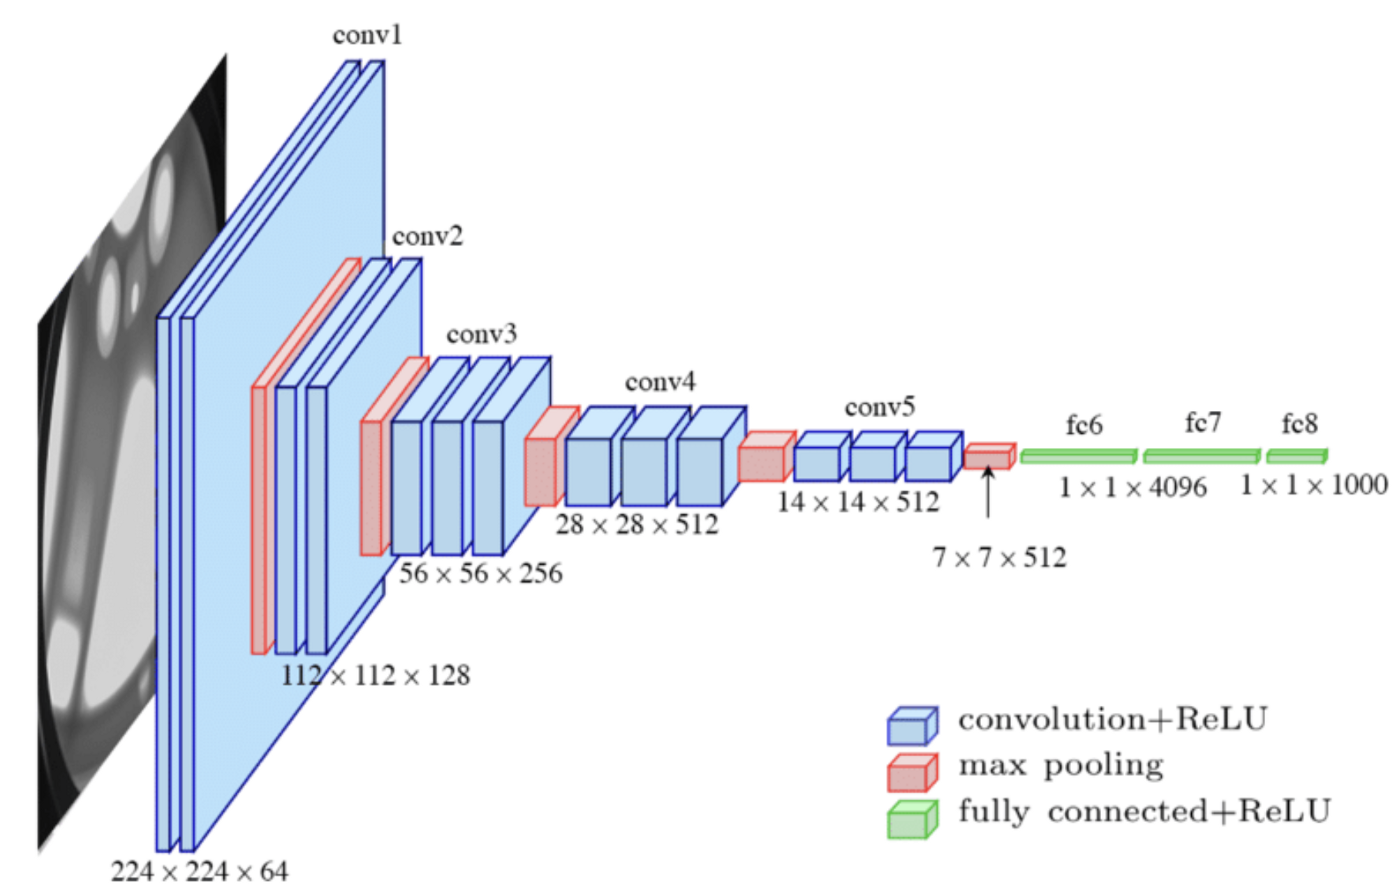
\includegraphics[width=0.8\textwidth]{presentation/figures-models/vgg16-model.png}
        \end{figure} 
\end{frame}
\begin{frame}{CNN: VGG16 shallow vs deep layer}

    \begin{minipage}[t]{.45\linewidth}  
    \begin{figure}
            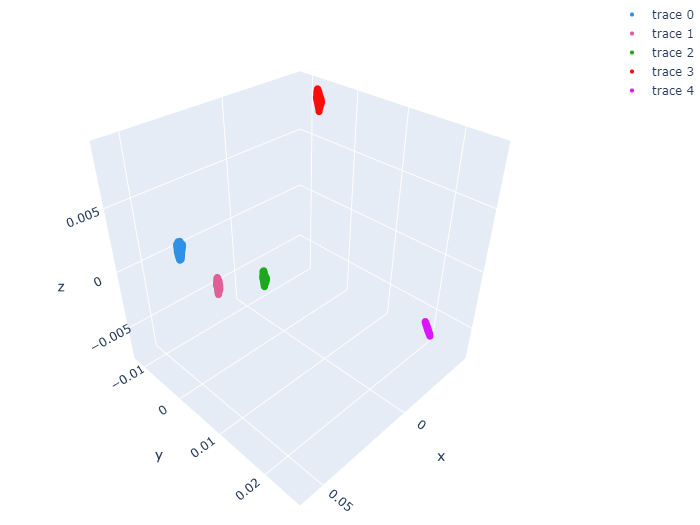
\includegraphics[width=\textwidth]{presentation/embeddings/VGG16-2D-block1.png}
             \caption{VGG16 block 1 neural manifold.}
        \end{figure} 
    \end{minipage}
      \begin{minipage}[t]{.45\linewidth}   
      \begin{figure}         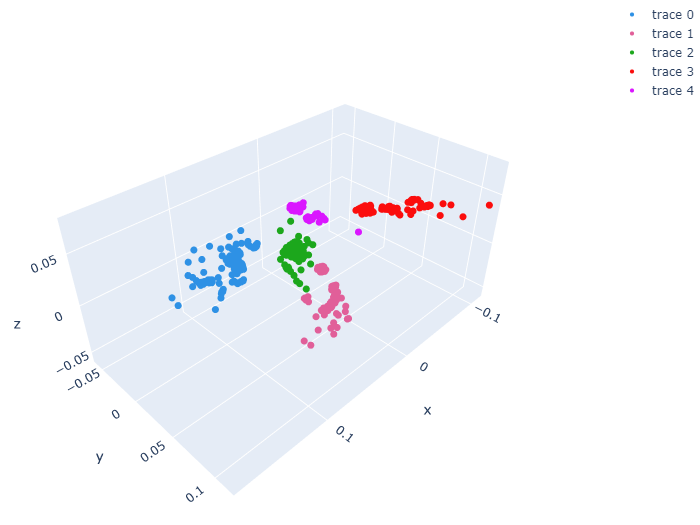
\includegraphics[width=\textwidth]{presentation/embeddings/VGG16-2D-block3.png}
      \caption{VGG16 block 3 neural manifold.}
            \end{figure} 
    \end{minipage}
\end{frame}

\begin{frame}{CNN: VGG16 preserving spatial order}
\begin{figure}
            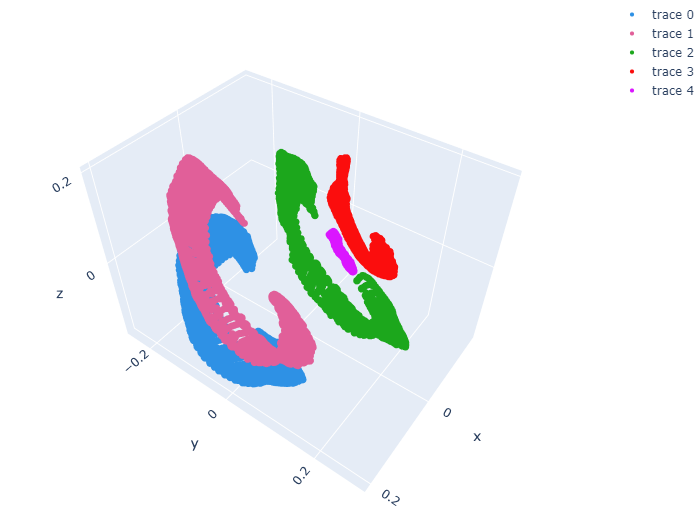
\includegraphics[width=0.4\textwidth]{presentation/embeddings/VGG16-3D-block1.png}
            \caption{VGG16 block 1 neural manifold with spatial order preserved.}
        \end{figure} 
    \begin{minipage}[t]{.45\linewidth}  
    \begin{figure}
            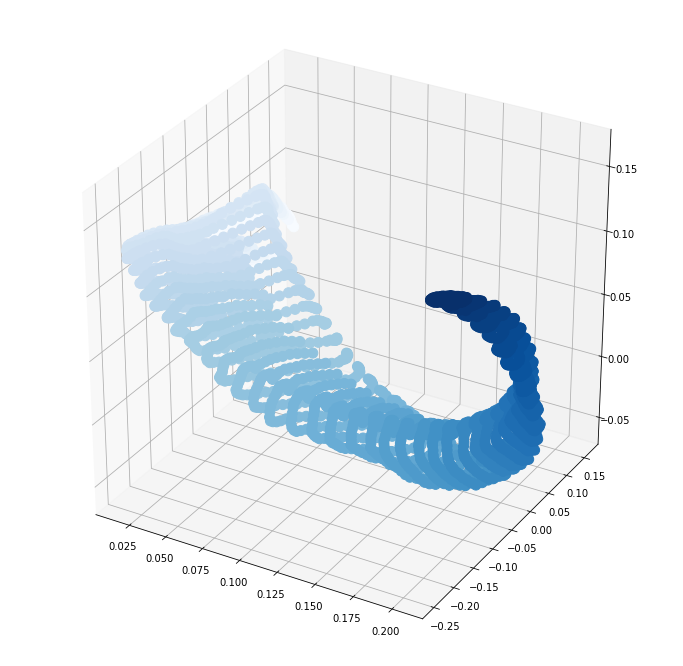
\includegraphics[width=0.5\textwidth]{presentation/embeddings/vgg16-spatial1.png}
            \caption{First cluster of neurons organized by vertical order.}
        \end{figure} 
    \end{minipage}
      \begin{minipage}[t]{.45\linewidth}   
      \begin{figure}         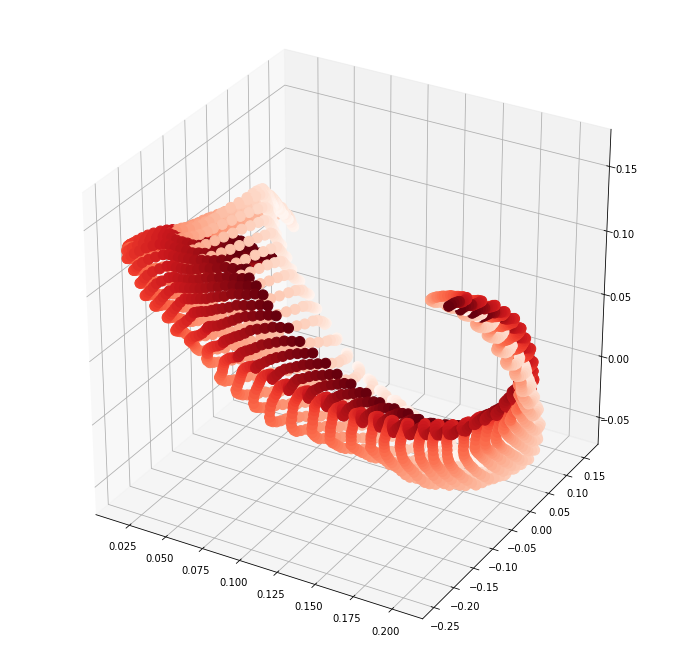
\includegraphics[width=0.5\textwidth]{presentation/embeddings/vgg16-spatial2.png}
      \caption{First cluster of neurons organized by horizontal order.}
            \end{figure} 
    \end{minipage}
\end{frame}
\begin{frame}{ViT structure}
Inspired by Transformer for NLP applications: an image is a sequence of 16-by-16 ``words."
      \begin{figure}[H]
        \centering
            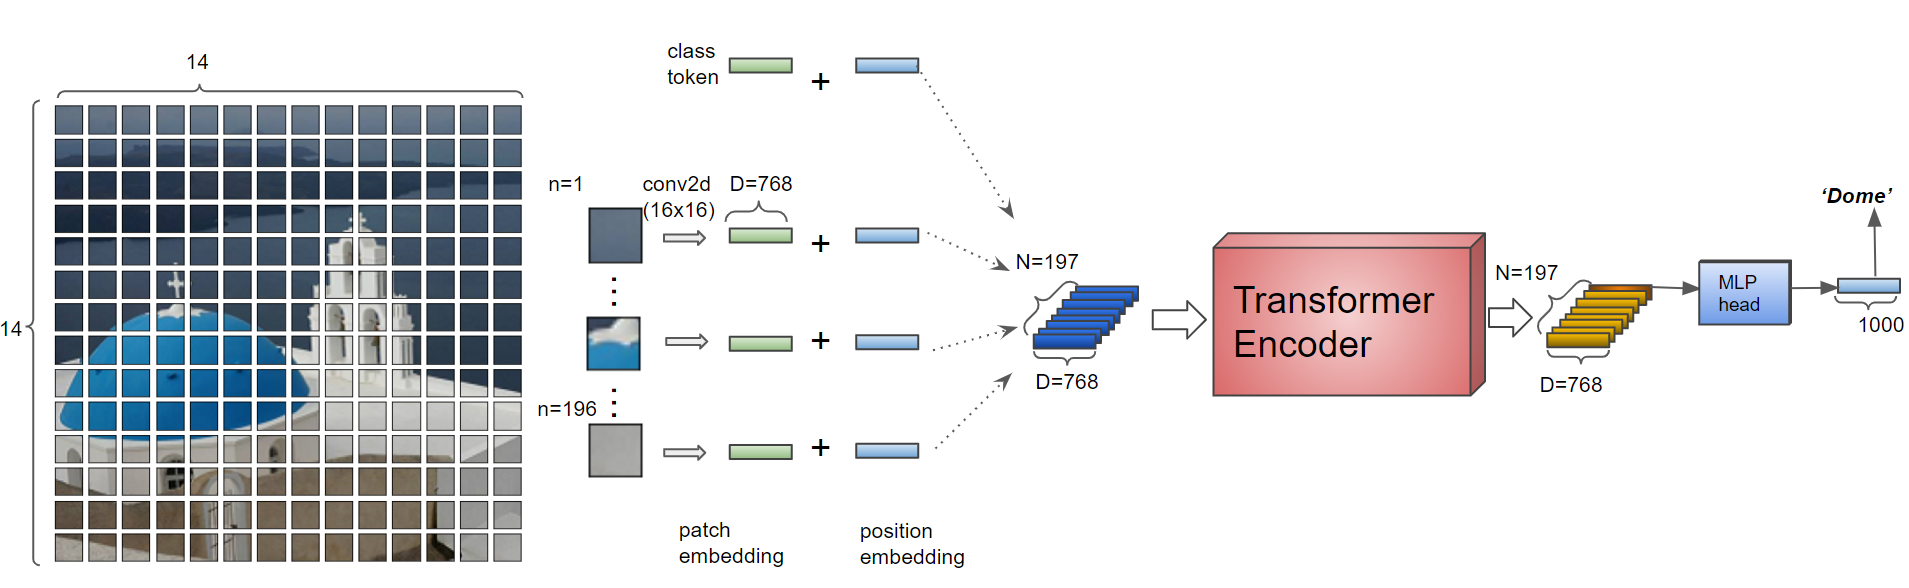
\includegraphics[width=\textwidth]{presentation/figures-models/vit_input.png}
        \end{figure} 
\end{frame}
\begin{frame}{ViT structure}
The key operation in ViT is \textit{self-attention}.
        \begin{figure}[H]
        \centering
            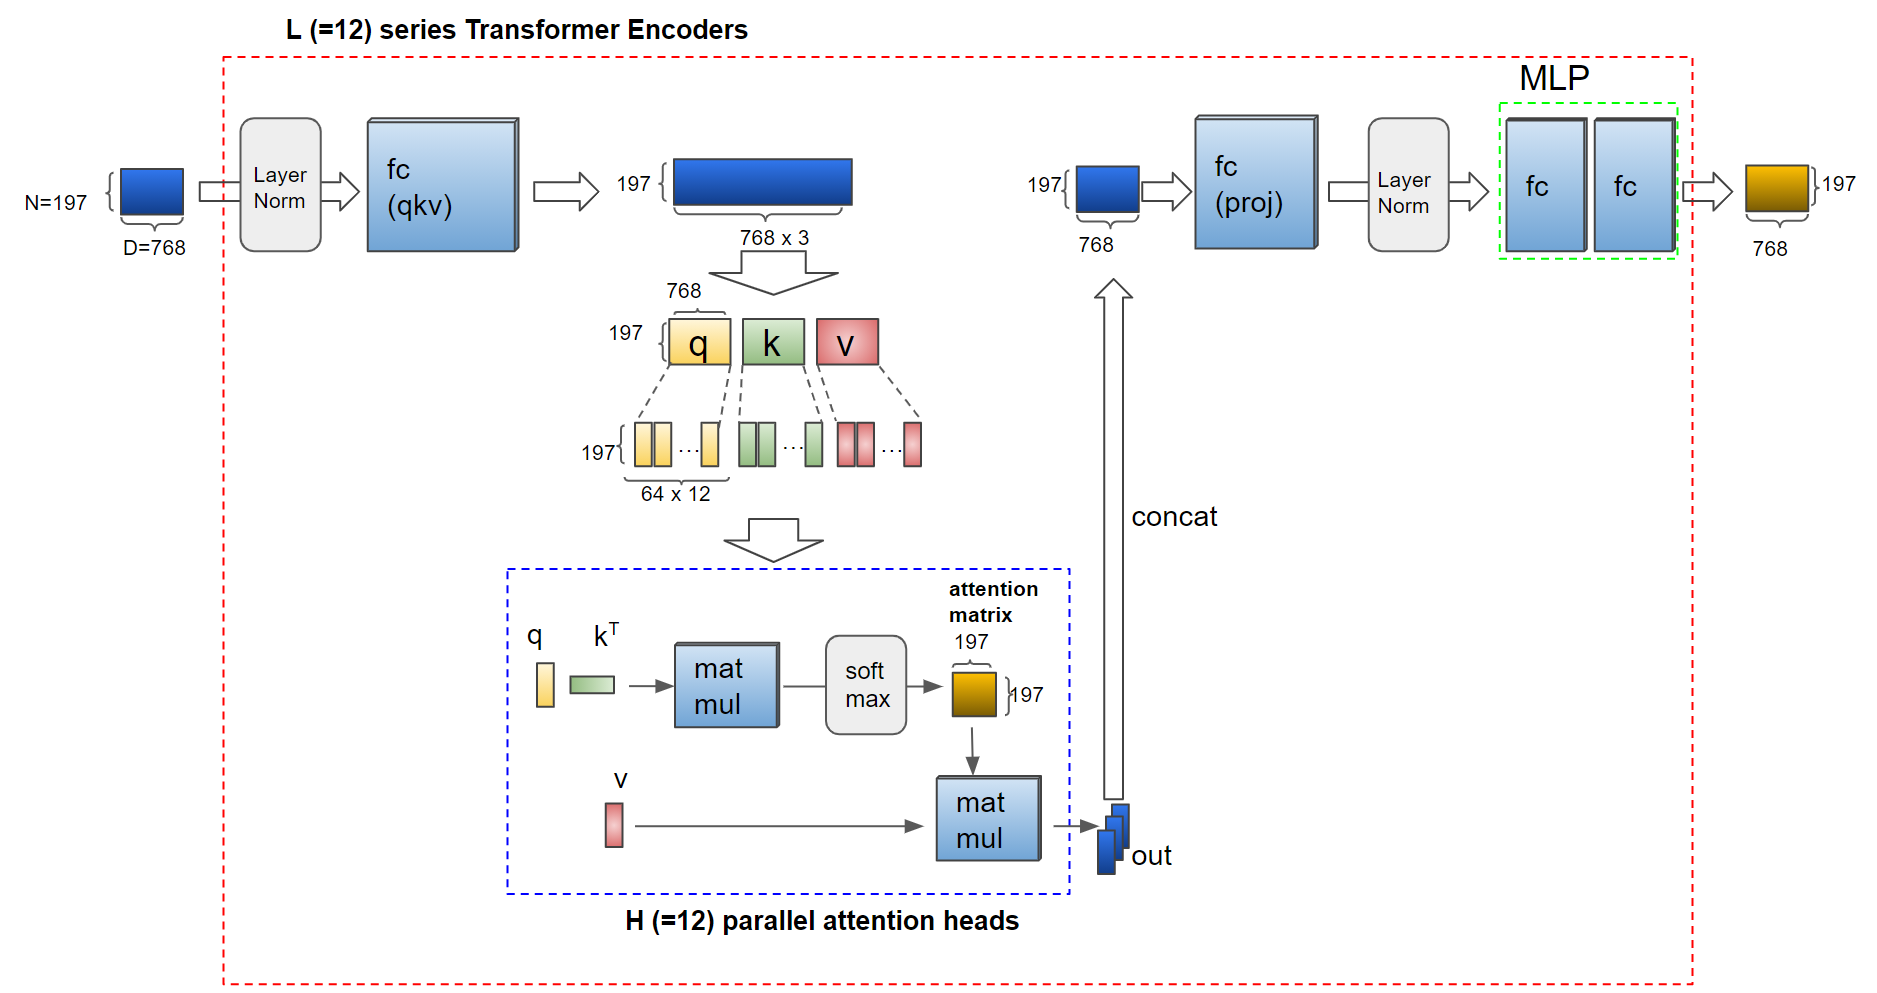
\includegraphics[width=\textwidth]{presentation/figures-models/vit_encoder.png}
        \end{figure} 
\end{frame}
\begin{frame}{Transformer: ViT shallow vs deep layer}
    \begin{minipage}[t]{.45\linewidth}  
    \begin{figure}
            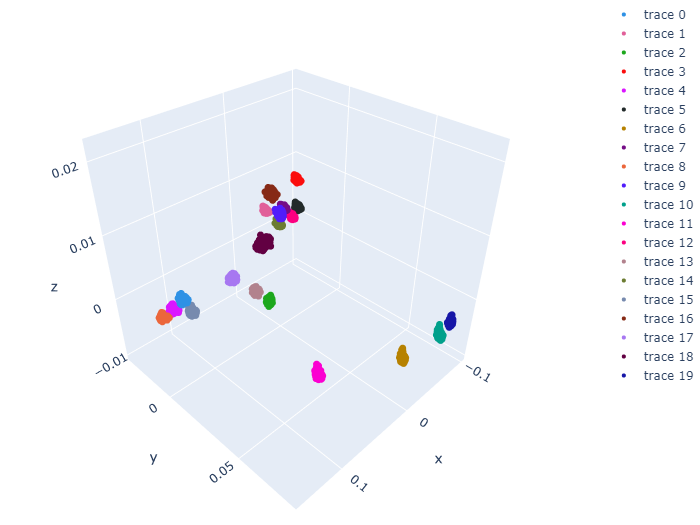
\includegraphics[width=\textwidth]{presentation/embeddings/vit-2d-layer1.png}
             \caption{ViT encoder layer 1 neural manifold.}
        \end{figure} 
    \end{minipage}
      \begin{minipage}[t]{.45\linewidth}   
      \begin{figure}         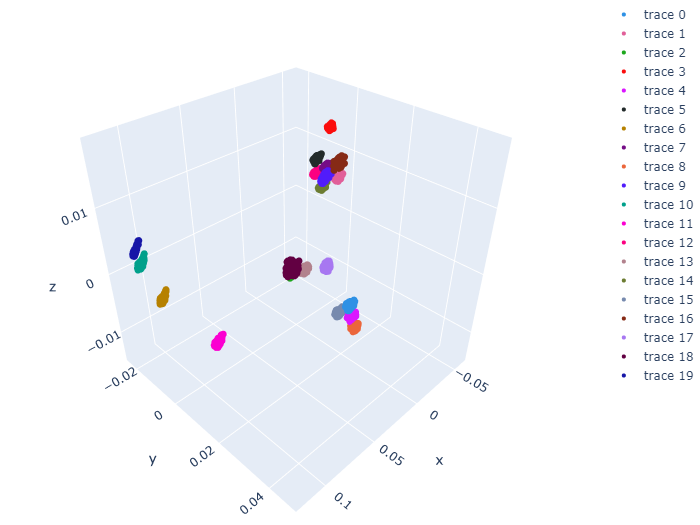
\includegraphics[width=0.9\textwidth]{presentation/embeddings/vit-2d-layer12.png}
       \caption{ViT encoder layer 12 neural manifold.}
            \end{figure} 
    \end{minipage}
\end{frame}
\begin{frame}{ViT preserving spatial order}
\begin{figure}
            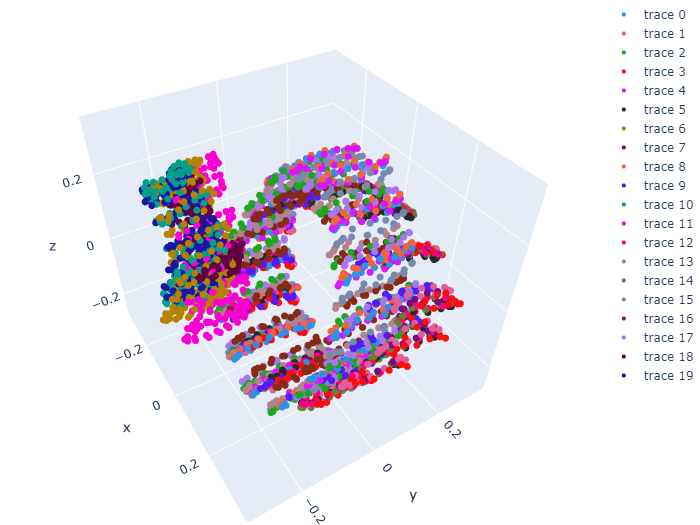
\includegraphics[width=0.4\textwidth]{presentation/embeddings/vit-3d-layer1.png}
            \caption{ViT encoder layer 1 neural manifold with spatial order preserved.}
        \end{figure} 
    \begin{minipage}[t]{.45\linewidth}  
    \begin{figure}
            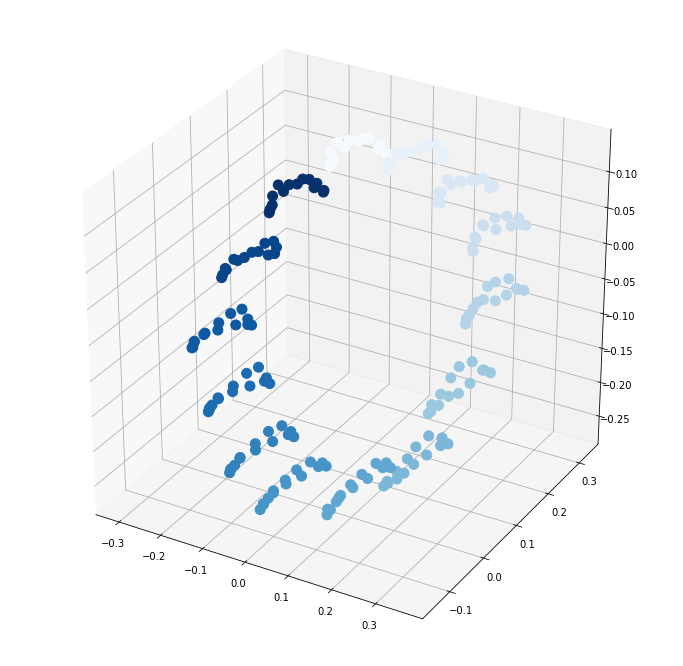
\includegraphics[width=0.5\textwidth]{presentation/embeddings/vit-spatial1.png}
            \caption{First cluster of neurons organized by vertical order.}
        \end{figure} 
    \end{minipage}
      \begin{minipage}[t]{.45\linewidth}   
      \begin{figure}         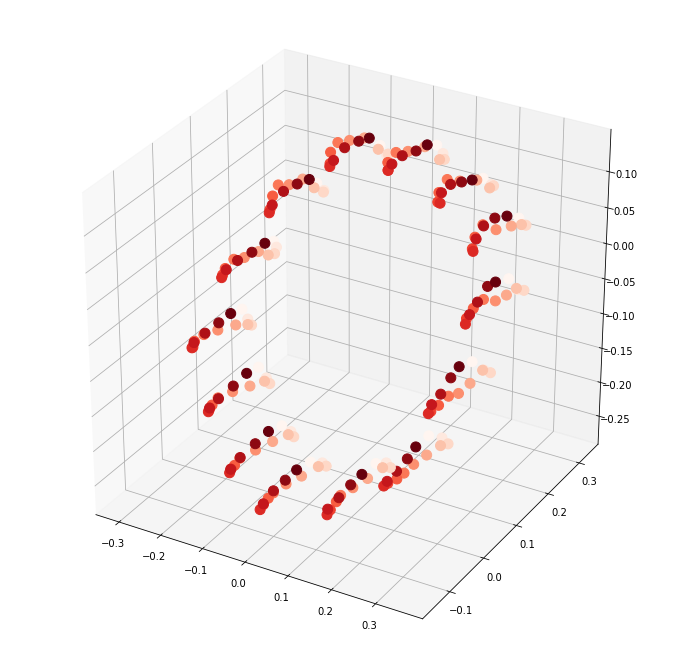
\includegraphics[width=0.5\textwidth]{presentation/embeddings/vit-spatial2.png}
      \caption{First cluster of neurons organized by horizontal order.}
            \end{figure} 
    \end{minipage}
\end{frame}
\begin{frame}{Compare neural manifolds}
        \begin{minipage}[t]{.45\linewidth}  
    \begin{figure}
            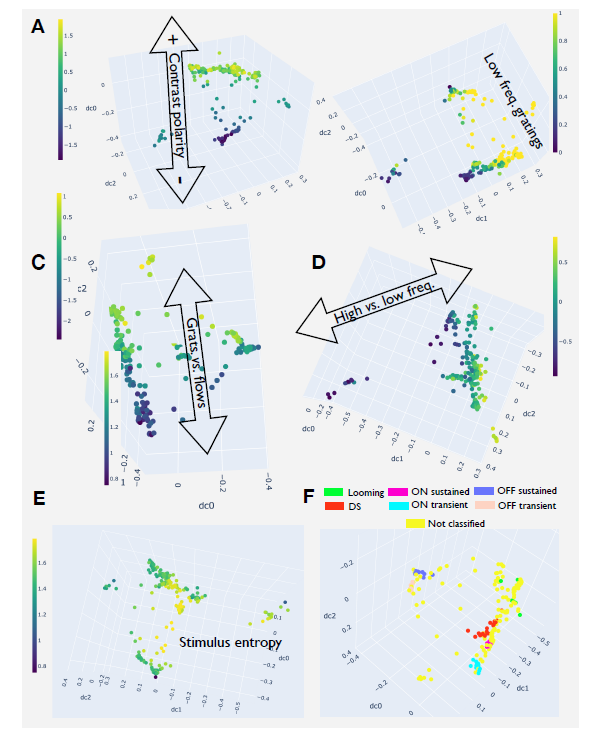
\includegraphics[width=0.45\textwidth]{presentation/embeddings/retina-manifold.PNG}
            \caption{Retina neural manifold. Adapted from \cite{dyballa_manifold_2021}.}
        \end{figure} 
    \end{minipage}
      \begin{minipage}[t]{.45\linewidth}   
      \begin{figure}         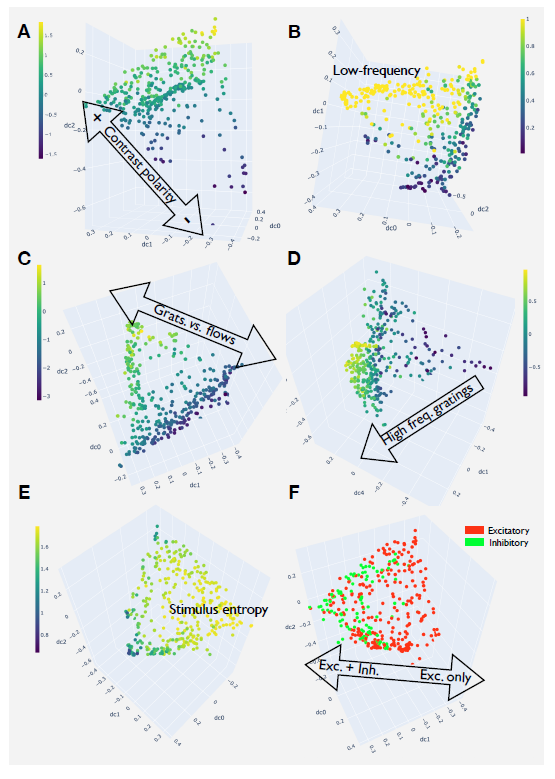
\includegraphics[width=0.4\textwidth]{presentation/embeddings/v1-manifold.PNG}
      \caption{V1 neural manifold. Adapted from \cite{dyballa_manifold_2021}.}
            \end{figure} 
    \end{minipage}
    
        \begin{minipage}[t]{.45\linewidth}  
    \begin{figure}
            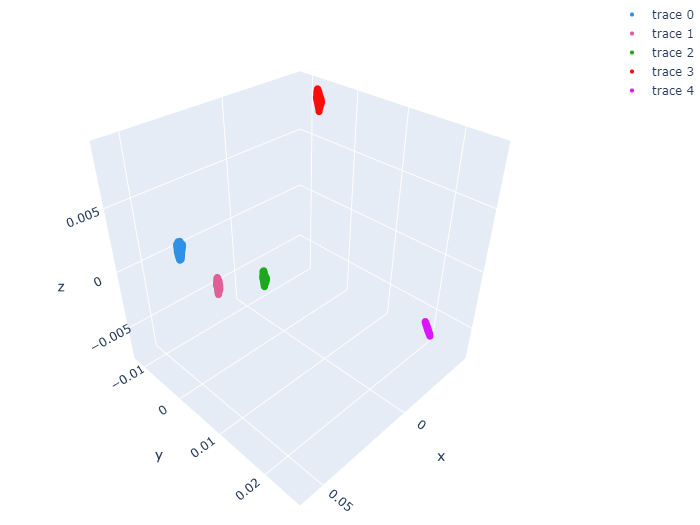
\includegraphics[width=0.5\textwidth]{presentation/embeddings/VGG16-2D-block1.png}
            \caption{VGG16 neural manifold.}
        \end{figure} 
    \end{minipage}
      \begin{minipage}[t]{.45\linewidth}   
      \begin{figure}         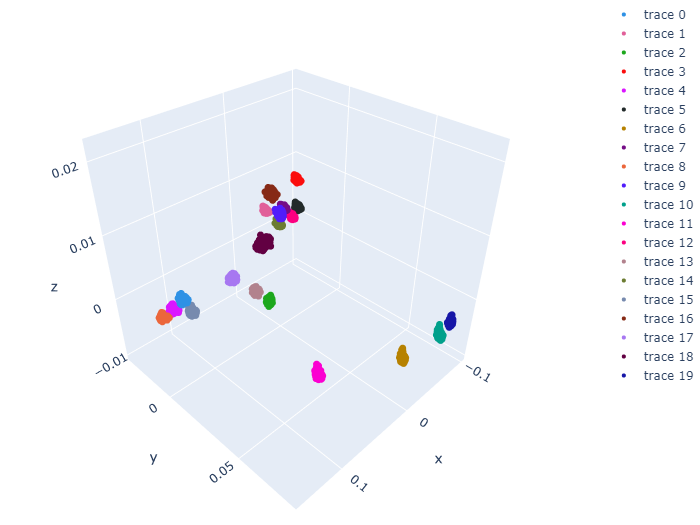
\includegraphics[width=0.5\textwidth]{presentation/embeddings/vit-2d-layer1.png}
      \caption{ViT neural manifold.}
            \end{figure} 
            
    \end{minipage}
\end{frame}
\begin{frame}{Compare mean flow ratios}
         \begin{figure}         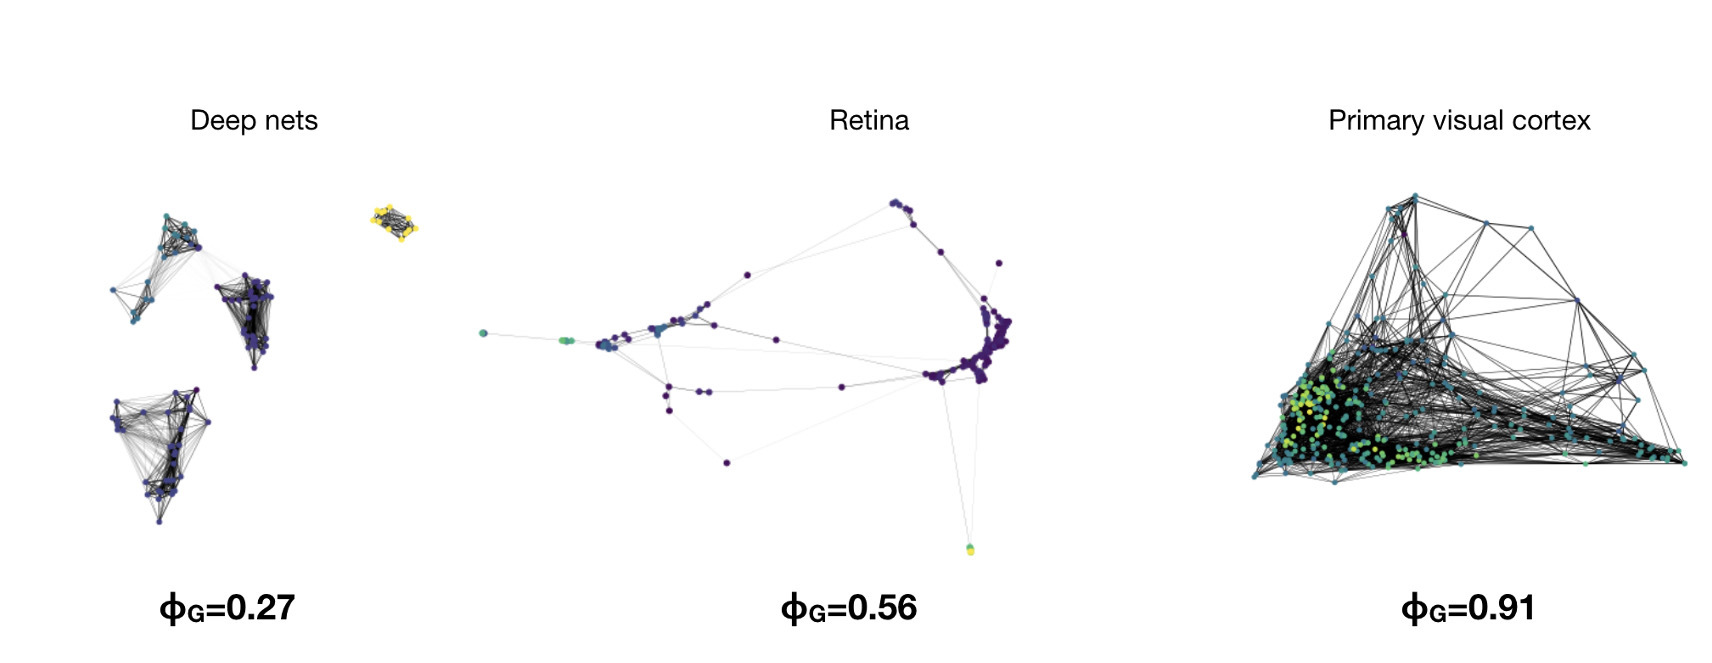
\includegraphics[width=\textwidth]{presentation/embeddings/mean-flow-ratio-results.jpg}
            \end{figure} 
\end{frame}

\begin{frame}{Concluding remarks}
    \begin{itemize}
        \item CNN and ViT are now the most popular models for image classification. 
        \item Both the convolution and self-attention mechanism give rise to discontinuous neural manifolds like the retina. 
        \item They are good enough as models for the retina, but are very bad models for V1. 
        \item What kind of computation can give rise to a more continuous neural manifold like V1?
        \item We are finishing up some experiments on RNN, which might give a partial answer. However, RNNs are rarely used for image classification.
    \end{itemize}
\end{frame}
\begin{frame}{Acknowledgements}
I would like to thank my supervisor Prof.~Francesca Spagnuolo  and co-supervisor and mentor Prof.~Steven W. Zucker and Dr.~Luciano Dyballa for their generous guidance and advice. They have made possible the many serendipitous moments in this project. 
\end{frame}
\section{References}
\begin{frame}{References}
\bibliographystyle{plain}
\bibliography{biblio}
\end{frame}

\end{document}